\documentclass{standalone}
\usepackage{amssymb}
\usepackage{tikz}
\usetikzlibrary{arrows.meta}
\usetikzlibrary{shapes.geometric,arrows,positioning}

\begin{document}

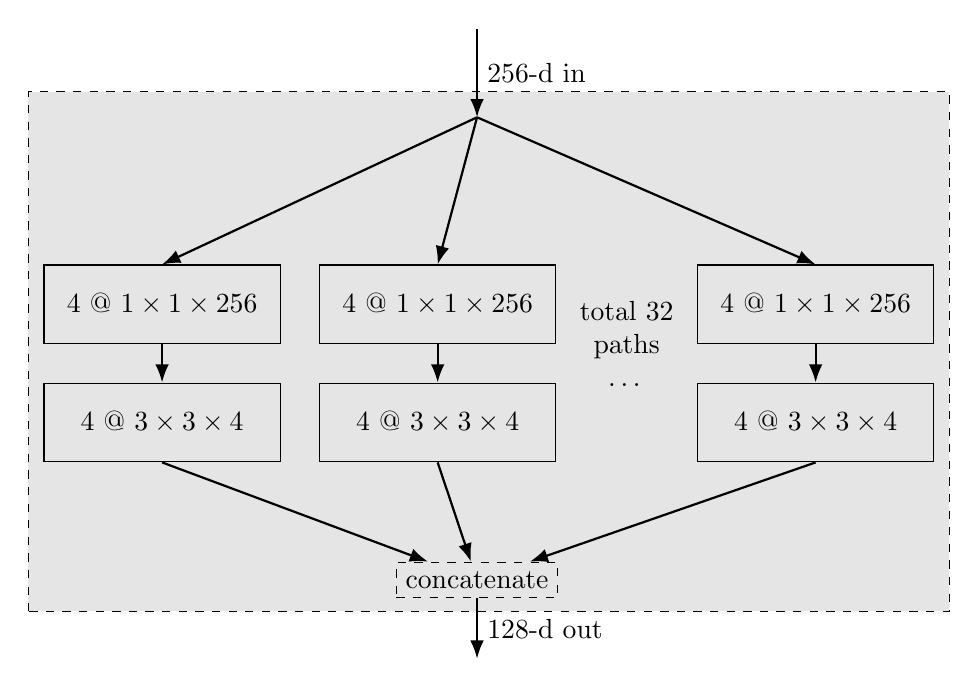
\begin{tikzpicture}
    \tikzstyle{conv-layer}=[draw,minimum width=3cm,minimum height=1cm]
    \tikzstyle{arrow}=[->, -Latex, thick]

    \draw[fill=black!10,dashed] (-4.2, -5.4) rectangle (7.5, 1.2);


    \node (input) at (1.5, 1) {};
    \path[arrow] (1.5, 2) edge node[right, midway] {$256$-d in} (input.south);
    \node[draw, dashed] (concatenate) at (1.5, -5) {concatenate};
    \node (between) at (3.4, -2.0) [align=center,text width=1.5cm] {total $32$ paths\\ \dots};
    \path[arrow] (concatenate.south) edge node[right, midway]  {$128$-d out} (1.5, -6);

    % first path
    \node (rect11) at (-2.5,-1.5) [conv-layer] {4 @ $1 \times 1 \times 256$};
    \node (rect12) at (-2.5,-3.0) [conv-layer] {4 @ $3 \times 3 \times 4$};
    \draw[arrow] (input.south) -- (rect11.north);
    \draw[arrow] (rect11.south) -- (rect12.north);
    \draw[arrow] (rect12.south) -- (concatenate);

    % second path
    \node (rect21) at ( 1,-1.5) [conv-layer] {4 @ $1 \times 1 \times 256$};
    \node (rect22) at ( 1,-3.0) [conv-layer] {4 @ $3 \times 3 \times 4$};
    \draw[arrow] (input.south) -- (rect21.north);
    \draw[arrow] (rect21.south) -- (rect22.north);
    \draw[arrow] (rect22.south) -- (concatenate);

    % last path
    \node (rect31) at ( 5.8,-1.5) [conv-layer] {4 @ $1 \times 1 \times 256$};
    \node (rect32) at ( 5.8,-3.0) [conv-layer] {4 @ $3 \times 3 \times 4$};
    \draw[arrow] (input.south) -- (rect31.north);
    \draw[arrow] (rect31.south) -- (rect32.north);
    \draw[arrow] (rect32.south) -- (concatenate);

\end{tikzpicture}
\end{document}
